\section{Non-submodular elastica}

\begin{frame}
\center
\huge
A quadratic non-submodular formulation for elastica

\vspace{2em}

\begin{minipage}{0.7\textwidth}
\normalsize
\begin{itemize}
\item{Global formulation attempt.}
\item{Fall back on a local formulation.}
\item{FlipFlow algorithm. Up to $10$x faster than LocalSearch.}
\end{itemize}
\end{minipage}

\end{frame}

\begin{frame}
{Non-submodular elastica}	
{Local models and completion effect}

\begin{minipage}[t][0.7\textheight][t]{1\textwidth}
\center

The completion effect can be difficult to recover in local formulations.\vspace{1em}

\only<2>{

\includegraphics[scale=0.5]{figures/non-submodular-elastica/completion/completion-1.png}
}%
\only<3>{
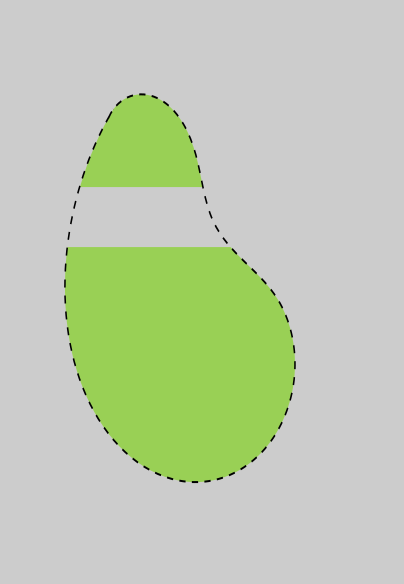
\includegraphics[scale=0.5]{figures/non-submodular-elastica/completion/completion-2.png}
}%
\only<4->{
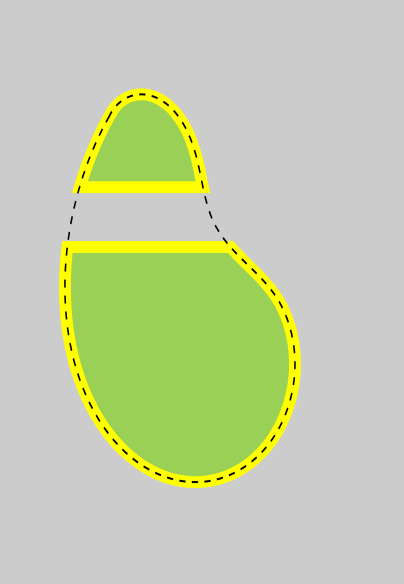
\includegraphics[scale=0.5]{figures/non-submodular-elastica/completion/completion-3.png}
}%
\vspace{1em}

\onslide<5->{Let's try a global formulation.}
\end{minipage}

\end{frame}

\begin{frame}
	{Non-submodular elastica}	
	{Difficulties with a global formulation}
\begin{minipage}[t][0.6\textheight][t]{1\textwidth}
\begin{minipage}{0.35\textwidth}
\only<1>{
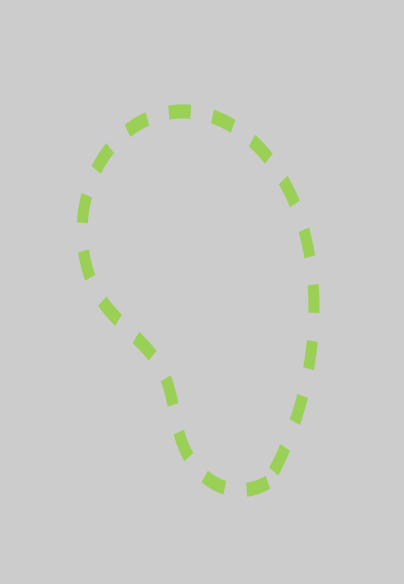
\includegraphics[scale=0.5]{figures/non-submodular-elastica/global/issues-2.png}
}
\only<2>{
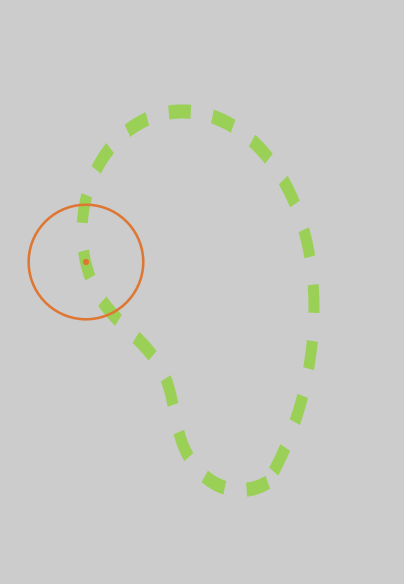
\includegraphics[scale=0.5]{figures/non-submodular-elastica/global/issues-3.png}
}
\only<3>{
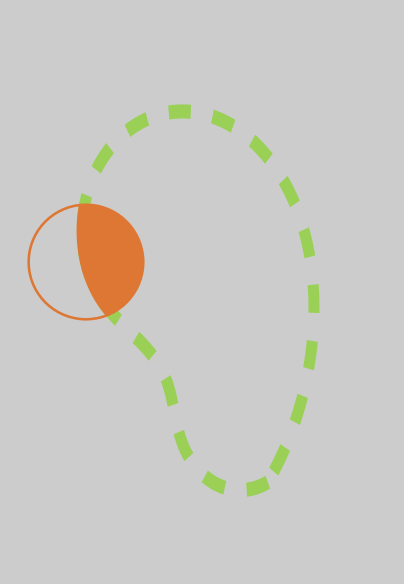
\includegraphics[scale=0.5]{figures/non-submodular-elastica/global/issues-4.png}
}
\only<4->{
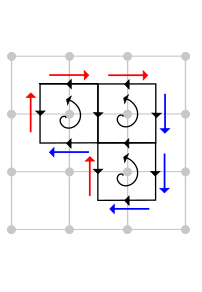
\includegraphics[scale=1]{figures/non-submodular-elastica/global/topological-constraints.png}
}
\end{minipage}
%
%
\begin{minipage}{0.64\textwidth}
\onslide<1->{
\begin{itemize}
	\onslide<1->{\item{$m$ pixels and $n$ edges.}}
	\onslide<2->{\item{Center of the estimation disk.}}
	\onslide<3->{\item{Pixel counting and estimation of curvature squared.}}
	\onslide<4->{\item{Linear topological constraints.}}	
	\onslide<5->{\item{Third order constrained non-convex binary problem.}}		
	\onslide<6->{\item{Level 1 linearization: non semi-definite positive quadratic problem.}}
	\onslide<7->{\item{Level 2 linearization: $O(m^3)$ variables.}}
\end{itemize}}
\end{minipage}	
\end{minipage}
%
%
\begin{minipage}[t][0.25\textheight][t]{1\textwidth}
\only<2>{
\begin{align*}
	\sum_{\ell_i \in \mathcal{L}}{ \vec{y}_i \left(\; \alpha + \beta \hat{\kappa}_{r}^2(D,\ell_i) \; \right)}\\\nonumber
\end{align*}}
\only<3>{
\begin{align*}
&\sum_{\ell_i \in \mathcal{L}}{ \vec{y}_i \left(\; \alpha + \frac{9}{r^6}\beta \big(c^2 - 2c\vec{A}_i^T\vec{x} + \vec{x}^T\vec{A}_i\vec{A}_i^T\vec{x}\big)\right)}\\
&\text{subject to} \quad \vec{x} \in \{0,1\}^m, \vec{y} \in \{0,1\}^n.
\end{align*}}
\only<4->{
\begin{align*}
&\sum_{\ell_i \in \mathcal{L}}{ \vec{y}_i \left(\; \alpha + \frac{9}{r^6}\beta \big(c^2 - 2c\vec{A}_i^T\vec{x} + \vec{x}^T\vec{A}_i\vec{A}_i^T\vec{x}\big)\right)}\\
&\text{subject to} \quad \vec{x} \in \{0,1\}^m, \vec{y} \in \{0,1\}^n, T(\vec{x},\vec{y}).
\end{align*}}
\end{minipage}

\end{frame}

\begin{frame}
{Non-submodular elastica}
{Simplification}
\center
$\hat{\kappa}(p) = \frac{3}{r^3}\left( \frac{\pi r^2}{2} - | B_r(p) \cap X | \right )$
\begin{minipage}[t][0.5\textheight]{1\textwidth}
\center
\only<1>{
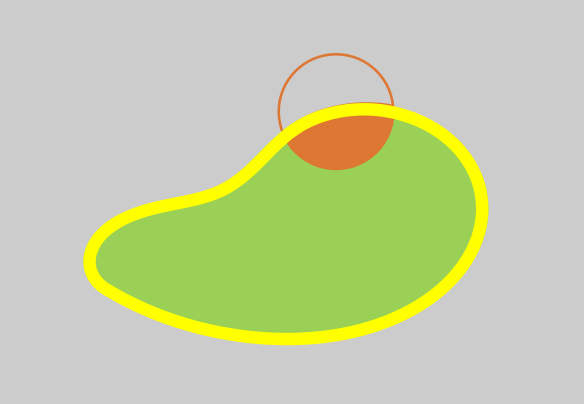
\includegraphics[scale=0.5]{figures/non-submodular-elastica/current-contour.png}}
\only<2>{
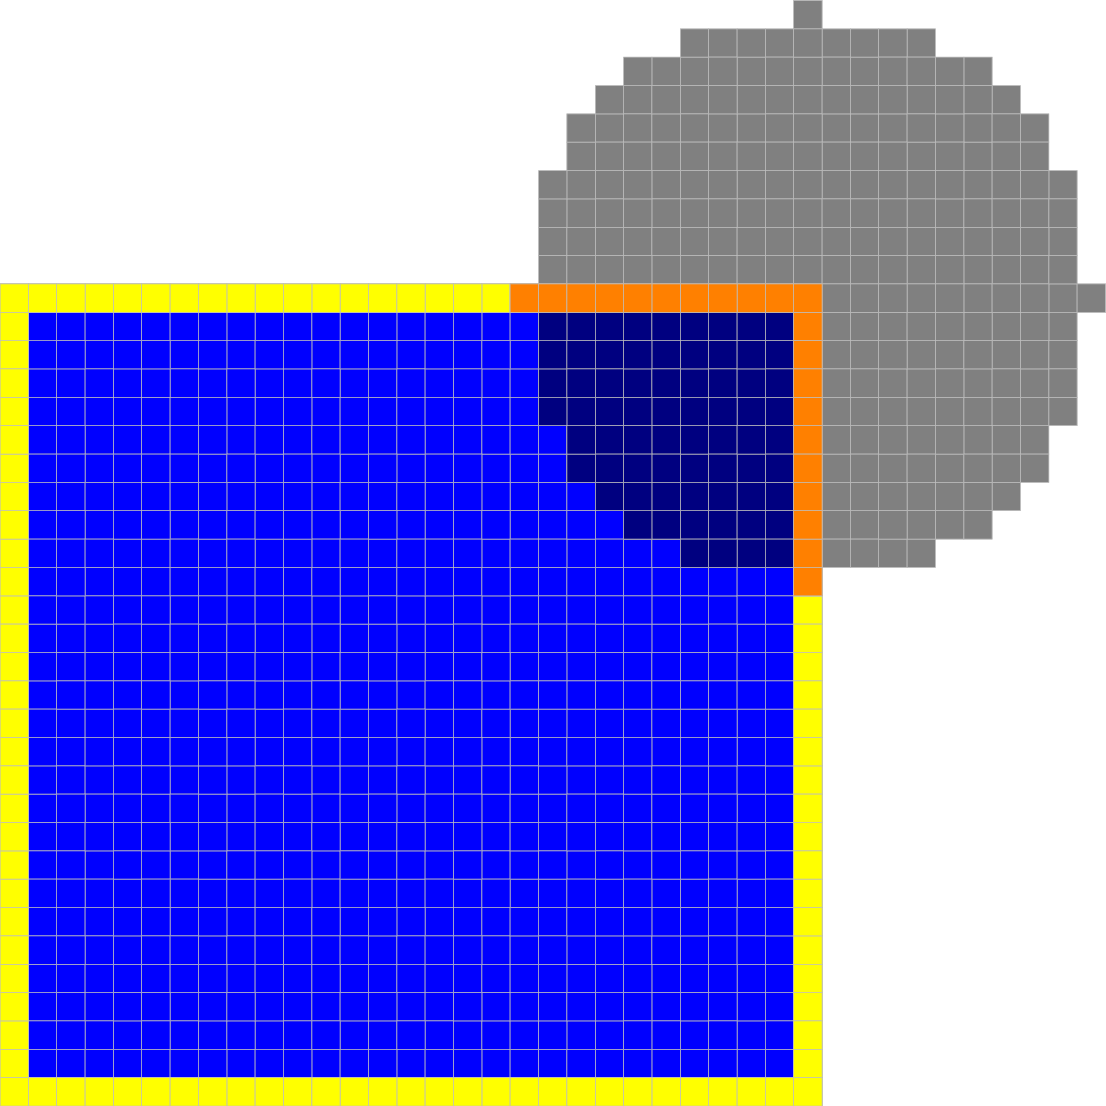
\includegraphics[scale=0.1]{figures/non-submodular-elastica/before-opt.png}\hspace{2em}
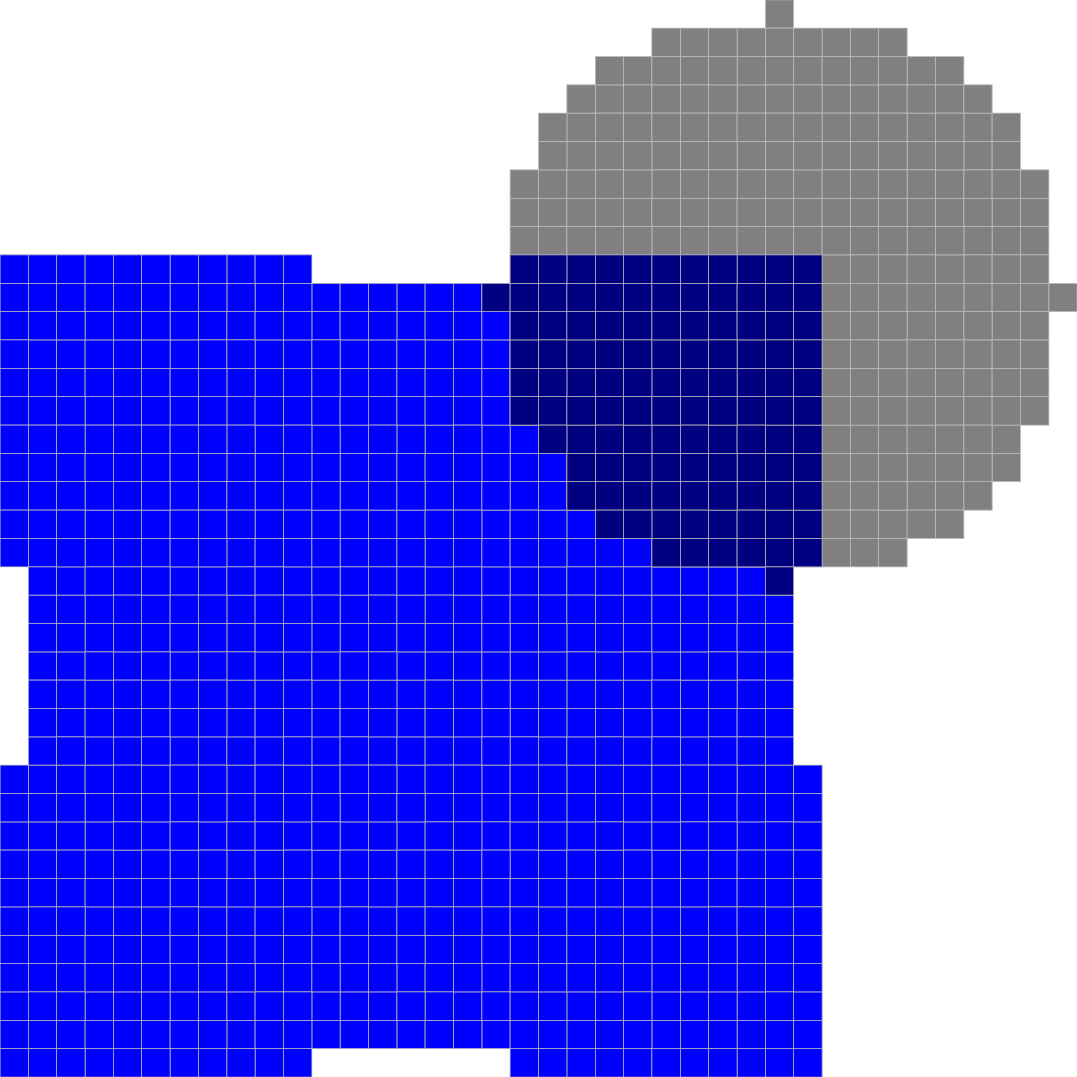
\includegraphics[scale=0.1]{figures/non-submodular-elastica/shape-opt-ball-after.png}}
\end{minipage}

\begin{itemize}
\item{Define the optimization region (yellow) as the inner contour of the shape, denoted $I$.}
\item{Evolve the estimation disks in the current contour.}
\item{Set pixels such that the curvature estimation is reduced.}
\end{itemize}
\end{frame}

\begin{frame}
{Non-submodular elastica}
{Simplification}
\center
$\hat{\kappa}(p) = \frac{3}{r^3}\left( \frac{\pi r^2}{2} - | B_r(p) \cap X | \right )$
\begin{minipage}[t][0.5\textheight]{1\textwidth}
\center
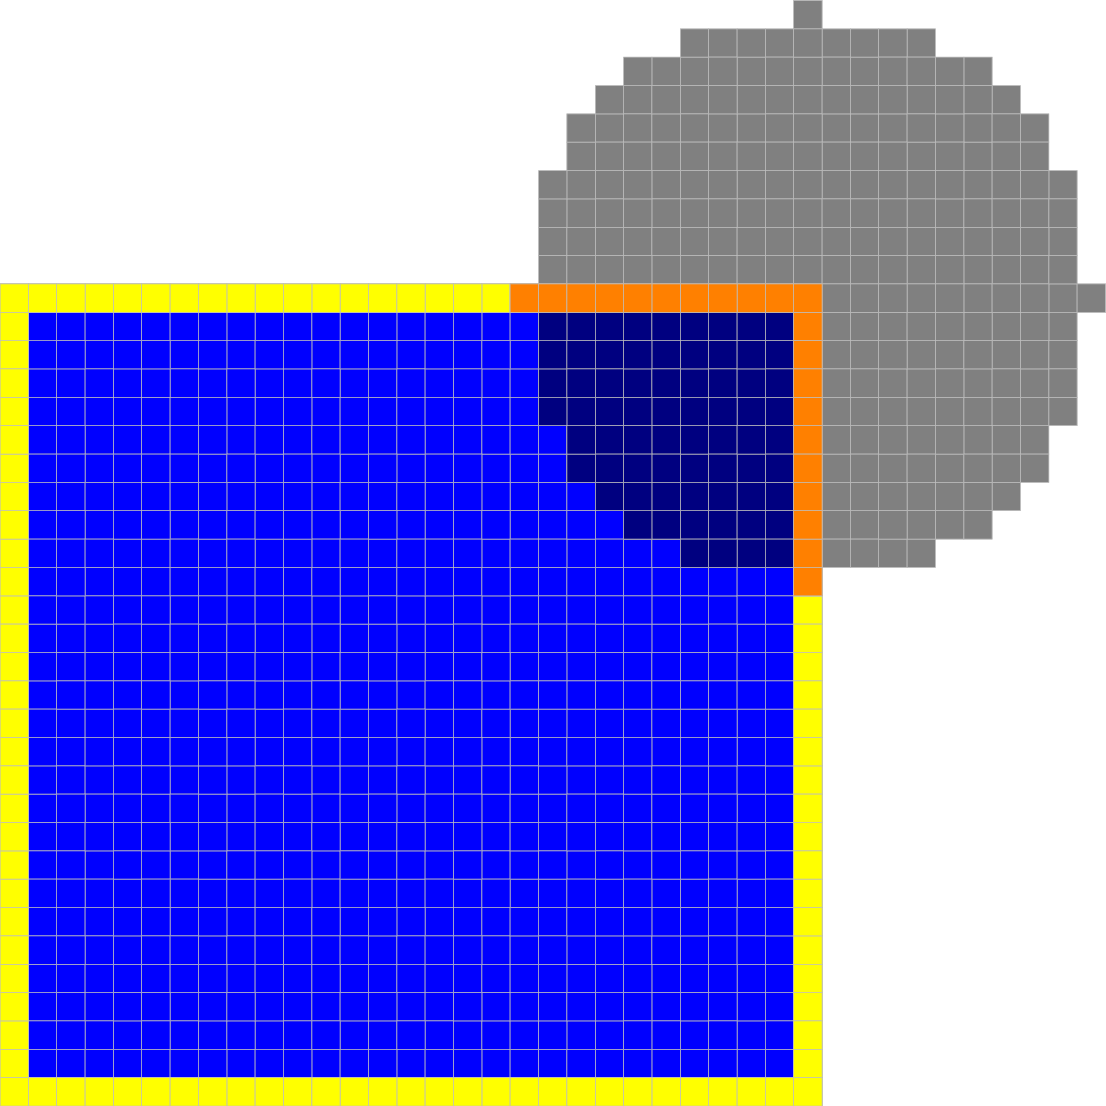
\includegraphics[scale=0.1]{figures/non-submodular-elastica/before-opt.png}\hspace{2em}
\only<1-2>{
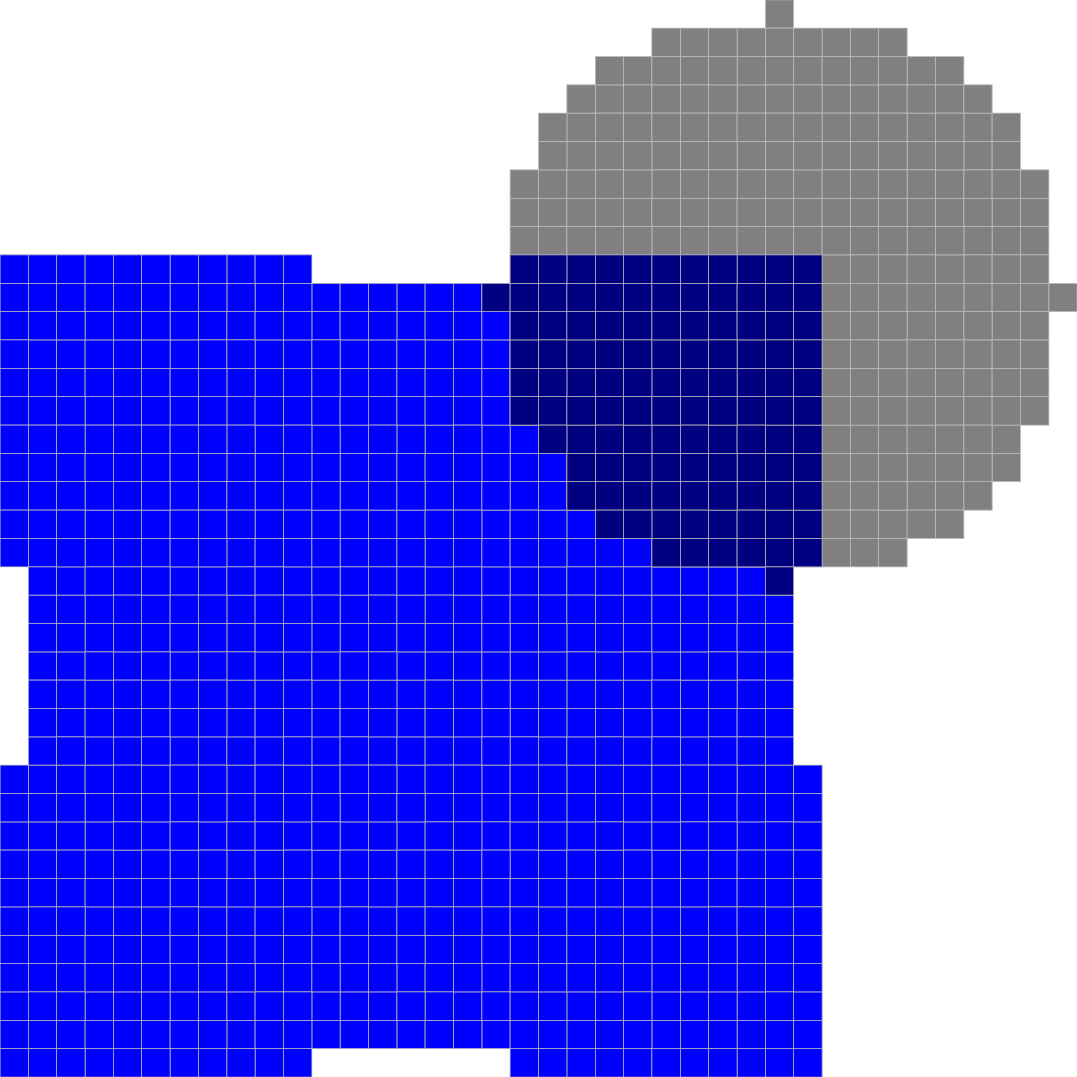
\includegraphics[scale=0.1]{figures/non-submodular-elastica/shape-opt-ball-after.png}}
\only<3>{
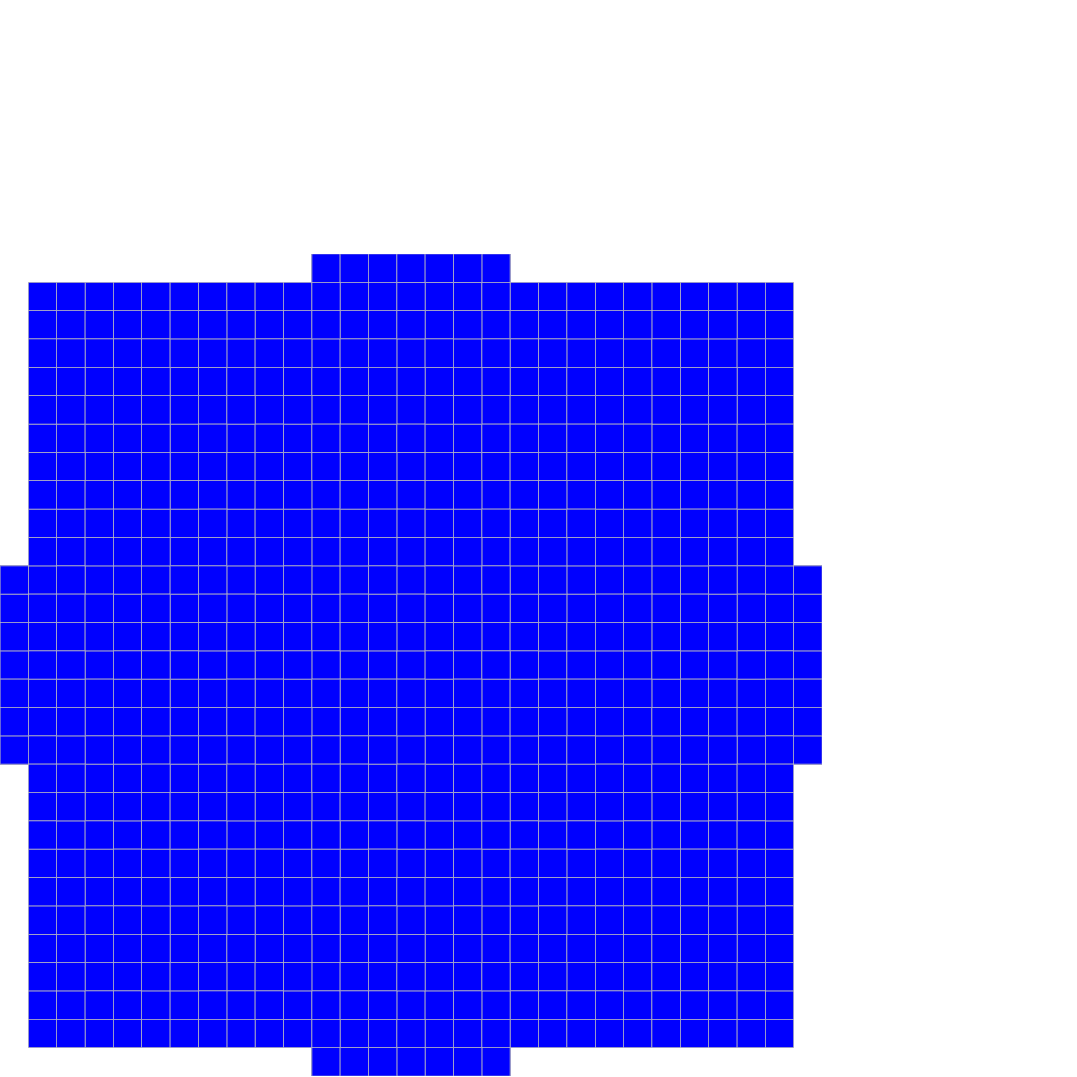
\includegraphics[scale=0.1]{figures/non-submodular-elastica/shape-opt-after-inverted.png}}
\end{minipage}

\begin{itemize}
\item{Optimization identifies zones of shortage (convex) or abundance (concave) of pixels.}
\onslide<2->{
\item{$x=1 \rightarrow$ Zone of shortage of pixels (convex) $\rightarrow$ Estimator disk should be shifted towards the interior $\rightarrow$ This pixel does not belong to the next contour. }}
\onslide<3->{\item{Therefore, we invert the optimal labeling.}}
\end{itemize}
\end{frame}

\begin{frame}
{Non-submodular elastica}
{FlipFlow}

\begin{minipage}[t][0.6\textheight][t]{1\textwidth}
\footnotesize

\begin{center}
$\displaystyle
D \subset \Omega \subset \mathbb{Z}^2, \quad
X^{(k)} := \{ \; x_i \in \{0,1\} \; | \; p_i \in \underbrace{I^{(k)}}_{\text{Inner contour}} \; \}$
\end{center}

\only<1-3>{
\begin{align*}
  E_{\vec{\theta}}^{flip}( \Ds^{(k)},X^{(k)} ) =& \sum_{ x_j \in X^{(k)}}{ \alpha s(x_j)} +  \sum_{ p \in I^{(k)}}{\beta \hat{\kappa}(p)^2}\\ 
  \onslide<2->{=& \sum_{ x_j \in X^{(k)}}{ \alpha \highlight{3}{1-2,4-}{s(x_j)}} \\
  +&\sum_{ \substack{p \in \\ I^{(k)}}}{ 2c_1 \beta  \Big( { (1/2+ |F_{r}^{(k)}(p)|-c_2) \cdot \sum_{ \substack{ x_j \in \\ X_{r}^{(k)}(p)}}{x_j} } + \sum_{ \substack{j<l, \\ x_j,x_l \in \\ X_{r}^{(k)}(p) } }{x_jx_l} \Big) }}
\end{align*}}
\only<4->{
\begin{align*}
  E_{\vec{\theta}}^{flip}( \Ds^{(k)}, \highlight{4}{1-3,5-}{1-X^{(k)}} ) =& \sum_{ x_j \in X^{(k)}}{ \alpha s(x_j)} +  \sum_{ p \in I^{(k)}}{\beta \hat{\kappa}(p)^2}\\ 
  =& \sum_{ x_j \in X^{(k)}}{ \alpha s(x_j)} \\
  +&\sum_{ p \in  I^{(k)}}{ 2c_1 \beta  \Big( { (1/2+ |F_{r}^{(k)}(p)|-c_2) \cdot \sum_{ \substack{ x_j \in \\ X_{r}^{(k)}(p)}}{x_j} } + \sum_{ \substack{j<l, \\ x_j,x_l \in \\ X_{r}^{(k)}(p) } }{x_jx_l} \Big) }
\end{align*}}
\end{minipage}%


\begin{minipage}[t][0.39\textheight][t]{1\textwidth}
\only<3>{
\begin{center}
\[
  \highlight{3}{1-2,4-}{s(x_j)}=\sum_{q_i \in \mathcal{N}_4(p_j)}{ t(q_i) }, \quad \text{where } t(q_i) = \left\{\begin{array}{ll}
  (x_j-x_i)^2, & \text{if } q_i \in I^{(k)}\\
  (x_j-1)^2, & \text{if } q_i \in F^{(k)}\\
  (x_j-0)^2, & \text{otherwise. }
  \end{array}\right.
\]
\end{center}}
\only<4>{
\begin{center}
\[
  s(x_j)=\sum_{q_i \in \mathcal{N}_4(p_j)}{ t(q_i) }, \quad \text{where } t(q_i) = \left\{\begin{array}{ll}
  (x_j-x_i)^2, & \text{if } q_i \in I^{(k)}\\
  (x_j-{\color{highlightcolor}0})^2, & \text{if } q_i \in F^{(k)}\\
  (x_j-{\color{highlightcolor}1})^2, & \text{otherwise. }
  \end{array}\right.
\]
\end{center}}%
%
%
\begin{minipage}{0.49\textwidth}
\scriptsize
\only<6->{\transparent{0.4}}
\only<5->{
\begin{center}
Shrink mode (convexities)
\[
\begin{array}{rl}
	a^{(k)} &\leftarrow \displaystyle \argmin_{X^{(k)}} E_{\vec{\theta}}^{flip}(D^{(k)},1-X^{(k)});\\[1.5em]
	D^{(k+1)} &\leftarrow F^{(k)} + a^{(k)}.
\end{array}
\]
\end{center}}
\end{minipage}%
%
%
\begin{minipage}{0.49\textwidth}
\scriptsize
\only<6->{
\begin{center}
Expansion mode (concavities)
\[
\begin{array}{rl}
	a^{(k)} &\leftarrow 	\displaystyle \argmin_{\overline{X}^{(k)}} E_{\vec{\theta}}^{flip}(\overline{D}^{(k)},1-\overline{X}^{(k)});\\[1.5em]
	D^{(k+1)} &\leftarrow \overline{ \overline{F}^{(k)} + a^{(k)} }.
\end{array}
\]
\end{center}}
\end{minipage}%
%
\end{minipage}
\end{frame}

\begin{frame}
{Non-submodular elastica}
{FlipFlow}

\begin{minipage}{0.49\textwidth}
\center
$r=3$\\
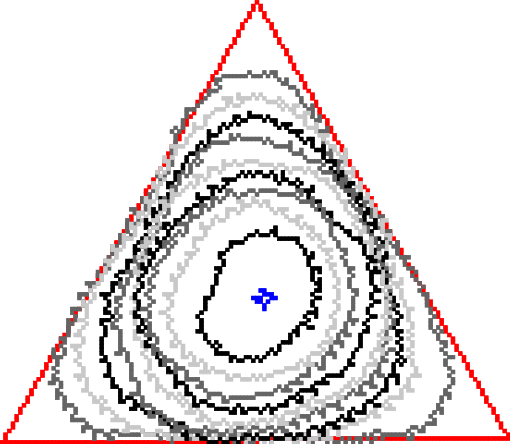
\includegraphics[scale=0.2]{figures/non-submodular-elastica/radius-effect/triangle-r3.png}\\[1em]
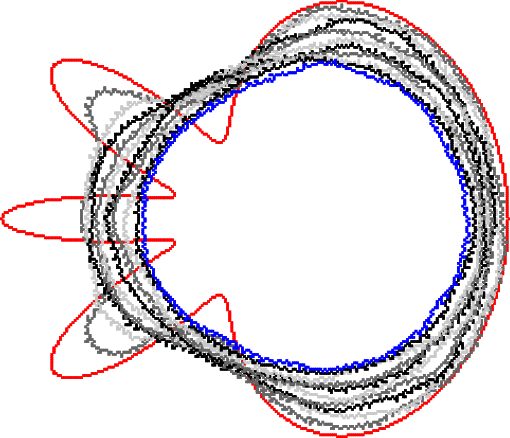
\includegraphics[scale=0.2]{figures/non-submodular-elastica/radius-effect/flower-r3.png}
\end{minipage}
\begin{minipage}{0.49\textwidth}
\center
$r=5$\\
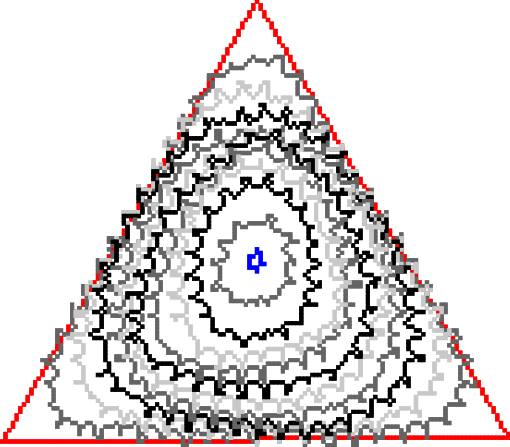
\includegraphics[scale=0.2]{figures/non-submodular-elastica/radius-effect/triangle-r5.png}\\[1em]
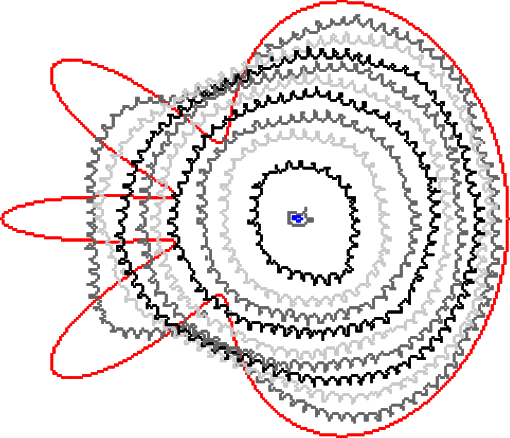
\includegraphics[scale=0.2]{figures/non-submodular-elastica/radius-effect/flower-r5.png}
\end{minipage}
\end{frame}

\begin{frame}
{Non-submodular elastica}
{Evaluation on farther rings}

\only<2->{
\footnotesize
\begin{align*}
  E_{(\vec{\theta},\highlight{2}{1,0}{m})}^{flip}( \Ds^{(k)},1-X^{(k)} ) =& \sum_{ x_j \in X^{(k)}}{ \alpha s(x_j)} +  \sum_{ p \in \highlight{2}{1,0}{R_m(\Ds^{(k)})}}{\beta \hat{\kappa}(p)^2}\\ 
  =& \sum_{ x_j \in X^{(k)}}{ \alpha s(x_j)} \\
  +&\sum_{ \substack{p \in \\ \highlight{2}{1,0}{R_m(\Ds^{(k)})}}}{ 2c_1 \beta  \Big( { (1/2+ |F_{r}^{(k)}(p)|-c_2) \cdot \sum_{ \substack{ x_j \in \\ X_{r}^{(k)}(p)}}{x_j} } + \sum_{ \substack{j<l, \\ x_j,x_l \in \\ X_{r}^{(k)}(p) } }{x_jx_l} \Big) }
\end{align*}

\begin{center}
$\displaystyle
\highlight{2}{1,0}{R_m(D)} := \{ p \; | \; m-1 < d_D(p) \leq m \} \cup \{ p \; | \; -m+1 > d_D(p) \geq -m \}$
\end{center}}

\only<1>{
	\begin{figure}
	\begin{tikzpicture}[overlay, remember picture] 
	\node at (current page.center) 
	    [
	    anchor=center,
	    xshift=0mm,
	    yshift=0mm
	    ] 
	{
	
	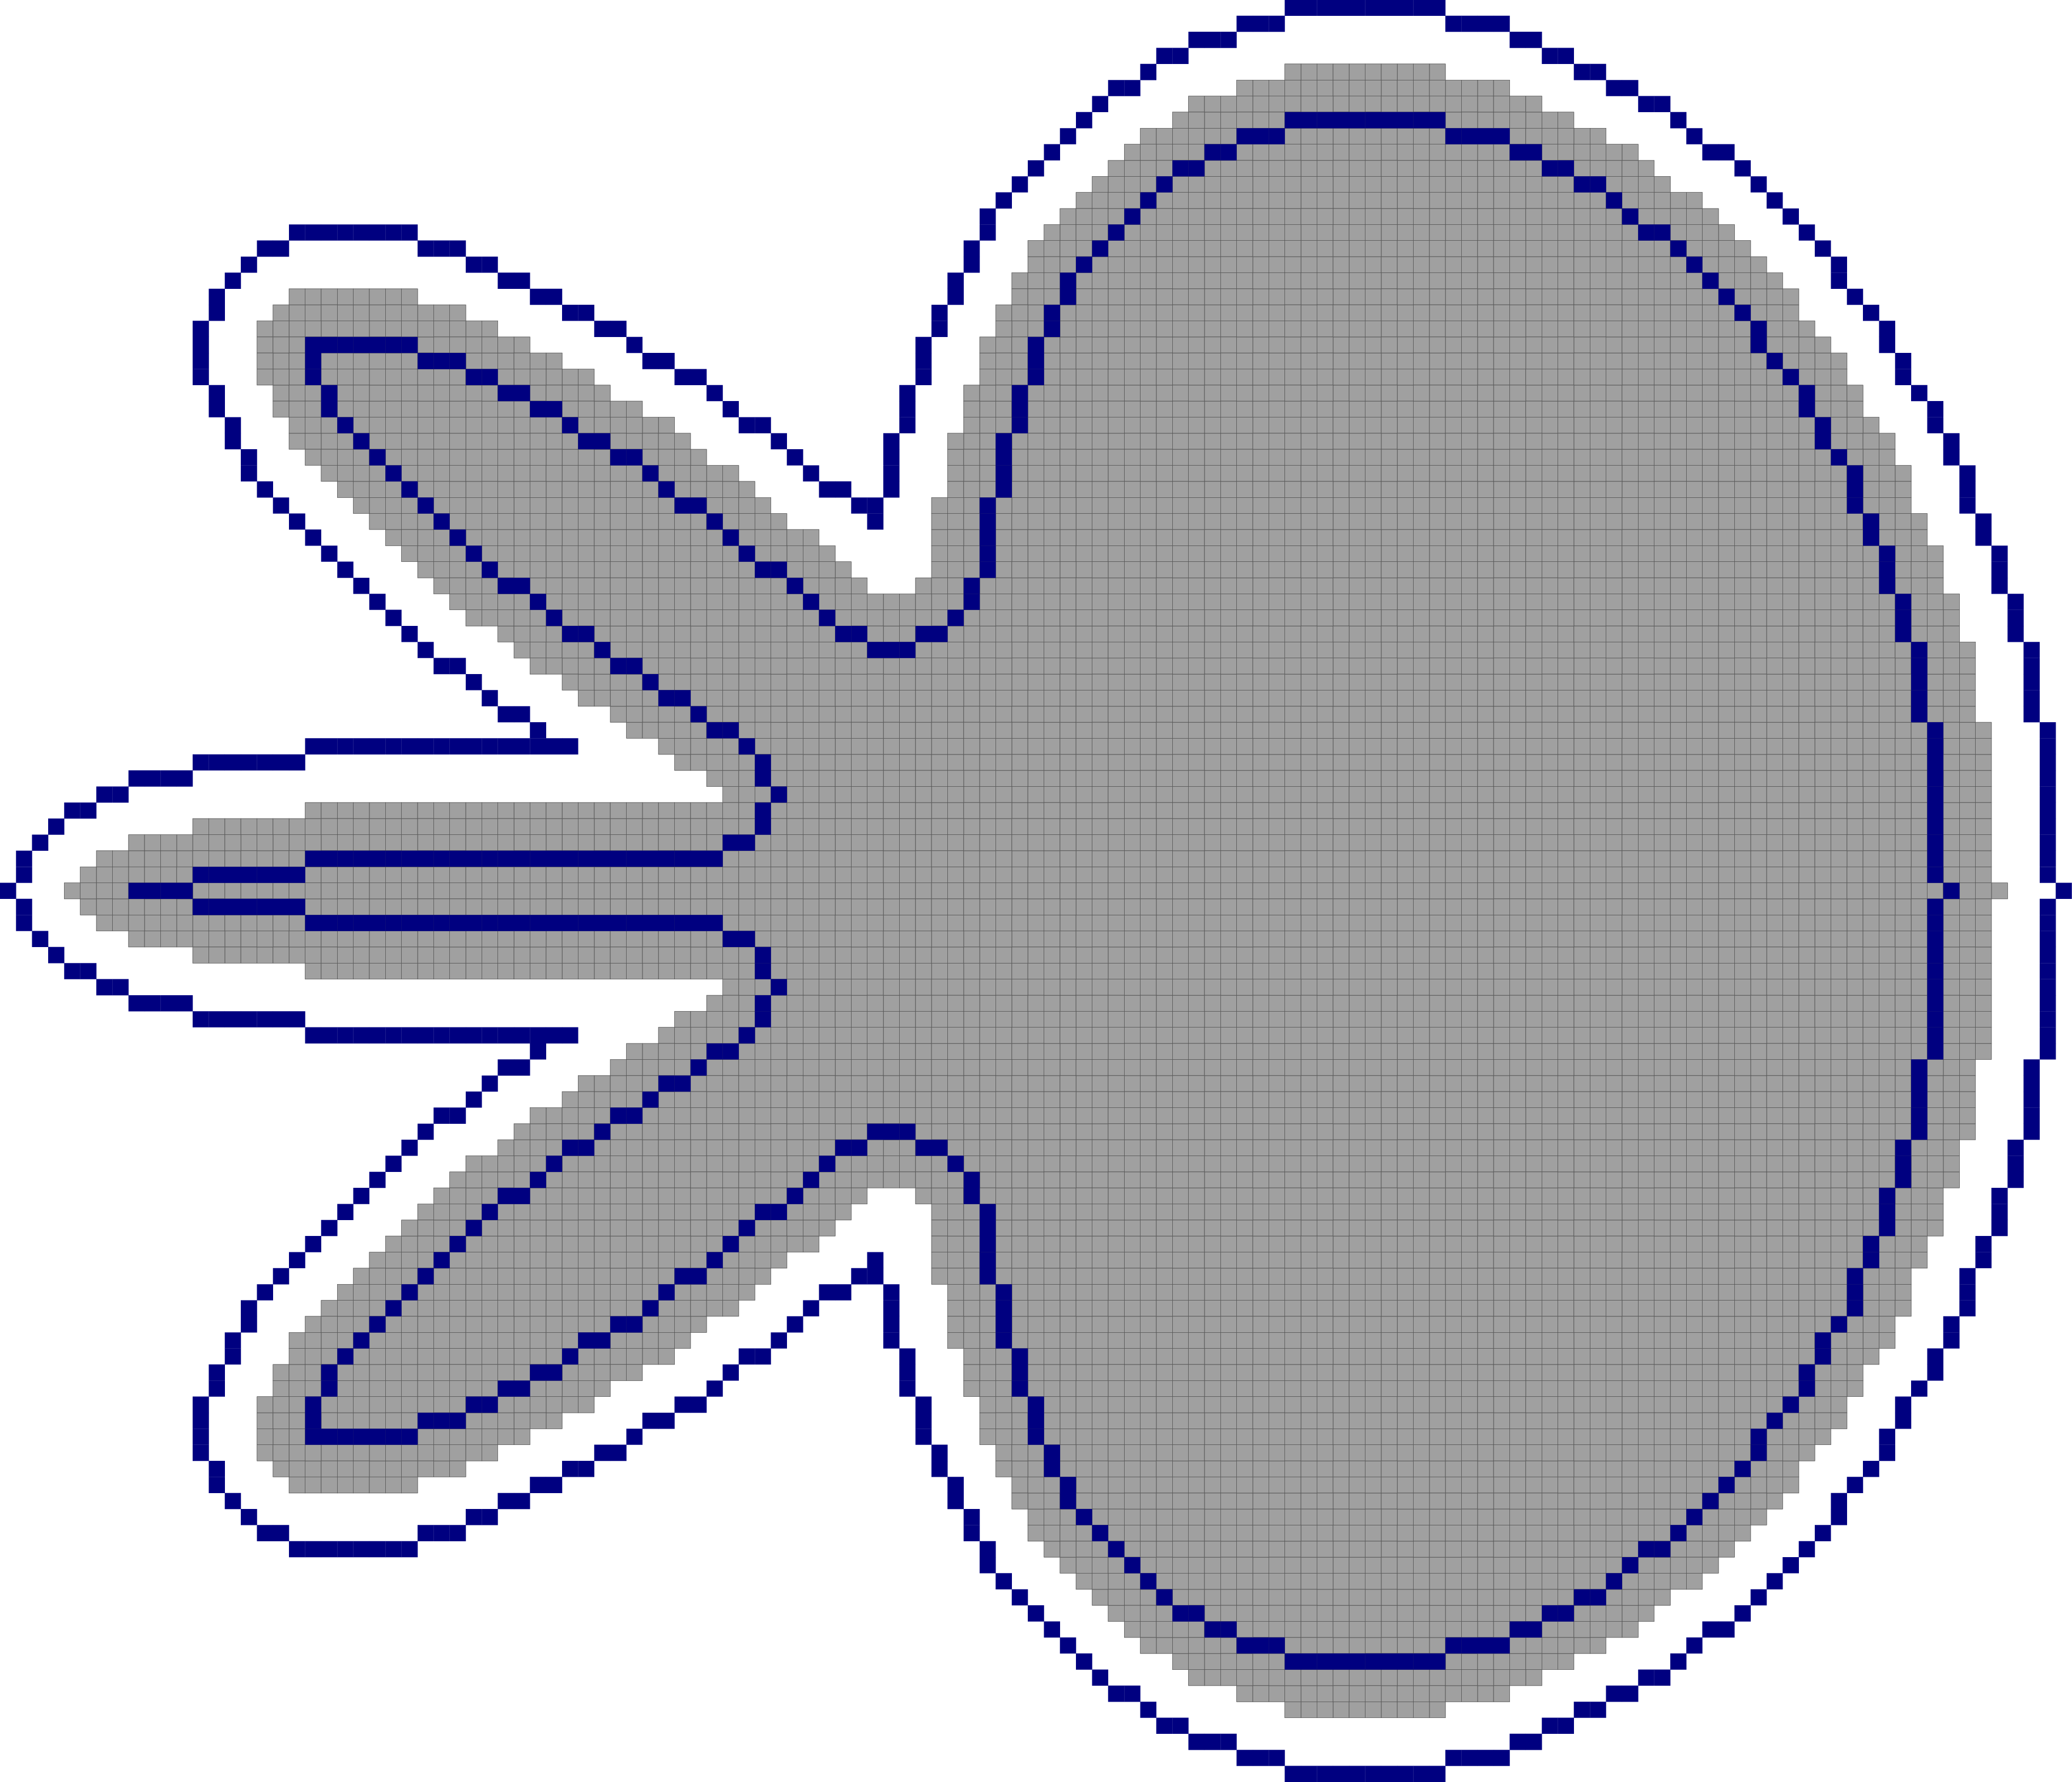
\includegraphics[scale=0.05]{figures/non-submodular-elastica/ring.png}
		
	};
	\end{tikzpicture}	
	\end{figure}}%
\end{frame}

\begin{frame}
{Non-submodular elastica}
{Evaluation on farther rings}
\begin{tabular}{cccc}
\multicolumn{4}{c}{$r=5$}\\
$m=1$ & $m=3$ & $m=4$ & $m=5$ \\
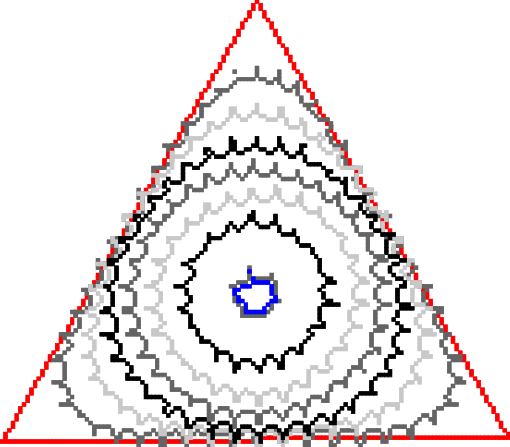
\includegraphics[scale=0.13]{figures/non-submodular-elastica/level-effect/triangle-l1.png}&
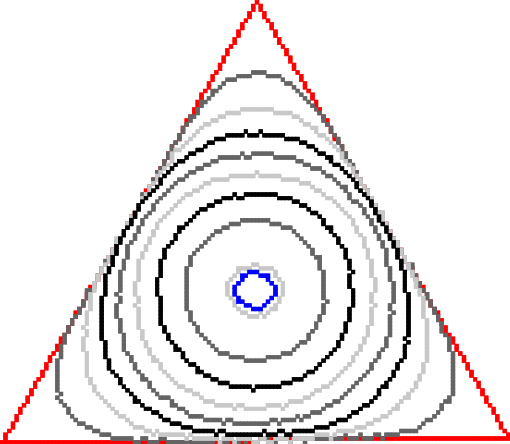
\includegraphics[scale=0.13]{figures/non-submodular-elastica/level-effect/triangle-l3.png}&
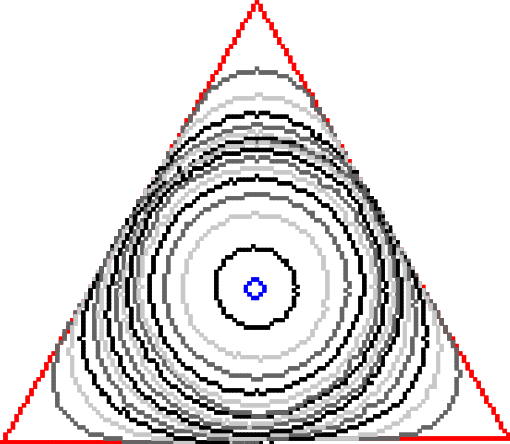
\includegraphics[scale=0.13]{figures/non-submodular-elastica/level-effect/triangle-l4.png}&
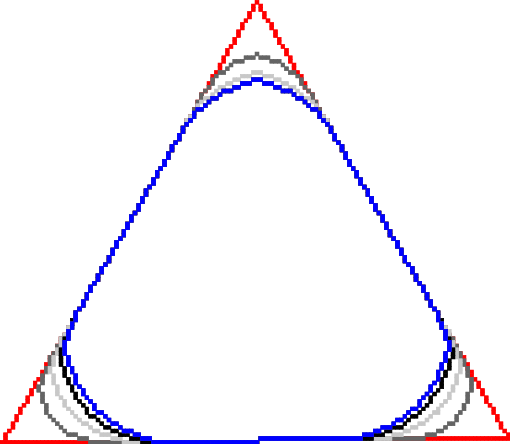
\includegraphics[scale=0.13]{figures/non-submodular-elastica/level-effect/triangle-l5.png}\\[2em]
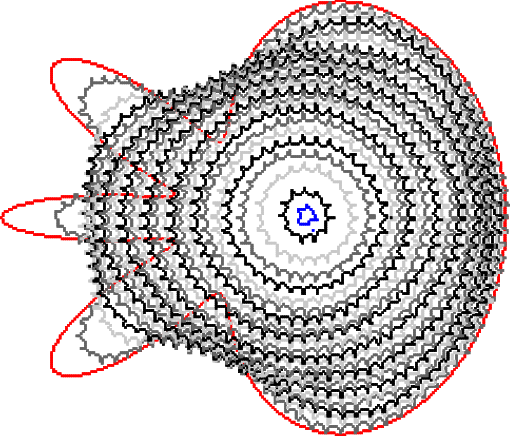
\includegraphics[scale=0.13]{figures/non-submodular-elastica/level-effect/flower-l1.png}&
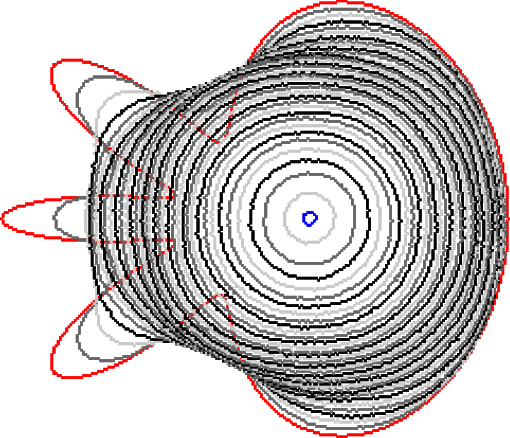
\includegraphics[scale=0.13]{figures/non-submodular-elastica/level-effect/flower-l3.png}&
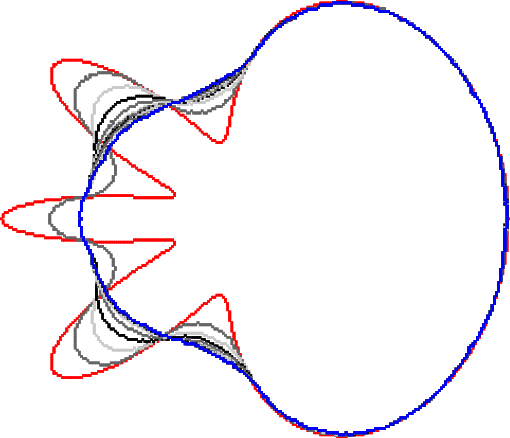
\includegraphics[scale=0.13]{figures/non-submodular-elastica/level-effect/flower-l4.png}&
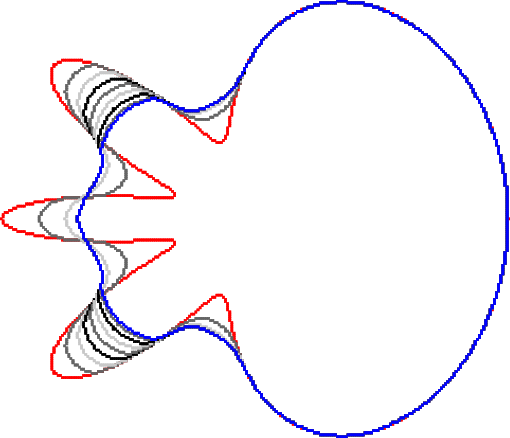
\includegraphics[scale=0.13]{figures/non-submodular-elastica/level-effect/flower-l5.png}
\end{tabular}
\end{frame}

\begin{frame}
{Non-submodular elastica}
{Contour correction}
\begin{tabular}{cc}
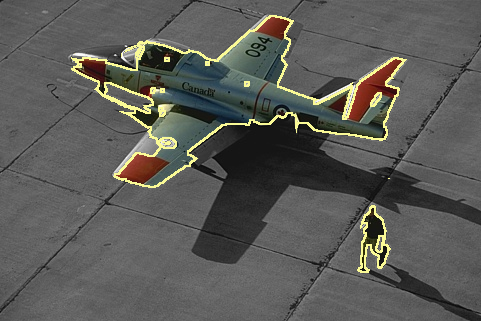
\includegraphics[scale=0.28]{figures/non-submodular-elastica/contour-correction/gc-seg-airplane.png}&
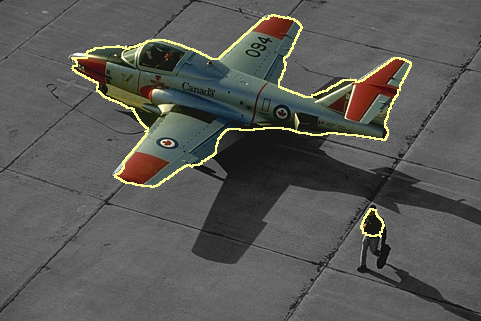
\includegraphics[scale=0.28]{figures/non-submodular-elastica/contour-correction/corrected-seg-airplane.png}\\[1em]
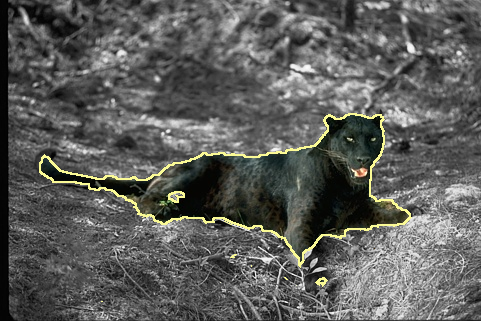
\includegraphics[scale=0.28]{figures/non-submodular-elastica/contour-correction/gc-seg-panther.png}&
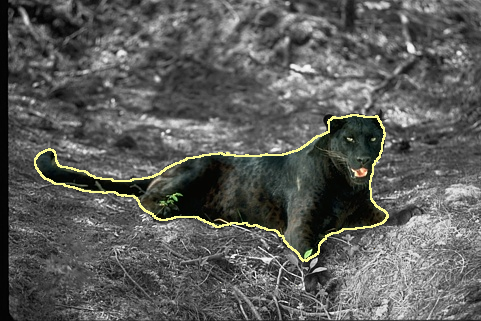
\includegraphics[scale=0.28]{figures/non-submodular-elastica/contour-correction/corrected-seg-panther.png}
\end{tabular}
\end{frame}

\begin{frame}
{Non-submodular elastica}
{Unlabeled ratio}
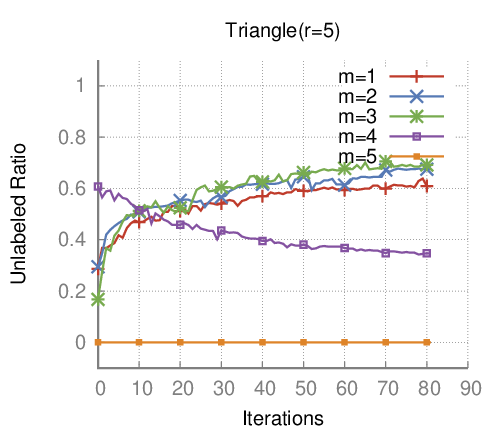
\includegraphics[scale=0.28]{figures/non-submodular-elastica/level-effect/plot-unlabeled-triangle.png}\hspace{1em}
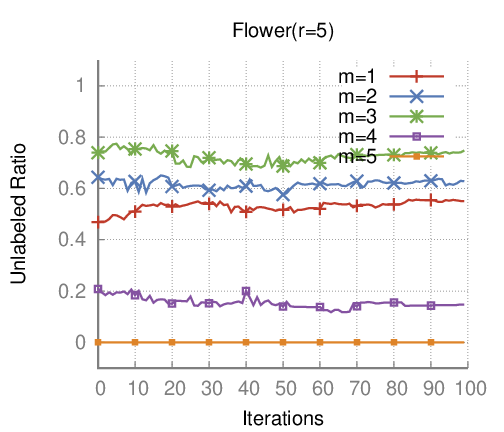
\includegraphics[scale=0.28]{figures/non-submodular-elastica/level-effect/plot-unlabeled-flower.png}

\begin{minipage}[t][0.5\textheight]{1\textwidth}
%
\only<2>{
\center
\begin{tabular}{cc}
$m=1$ & $m=3$\\[1em]
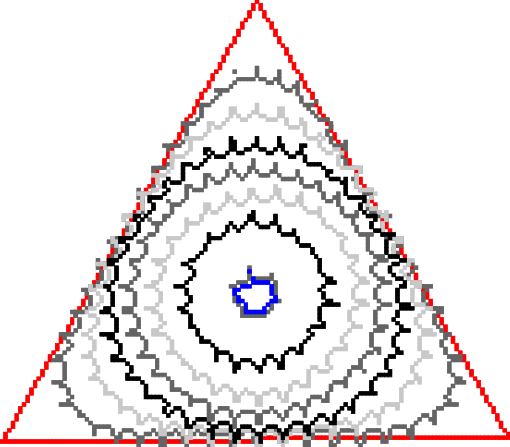
\includegraphics[scale=0.13]{figures/non-submodular-elastica/level-effect/triangle-l1.png}&
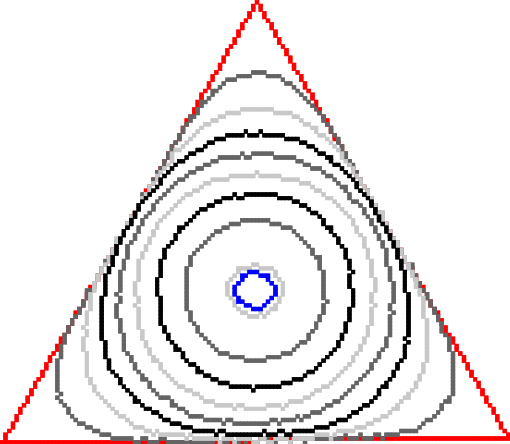
\includegraphics[scale=0.13]{figures/non-submodular-elastica/level-effect/triangle-l3.png}
\end{tabular}}%
%
\only<3>{
\begin{itemize}
\item{Unlabeled ratio is not sufficient to explain the smoothness at farther rings.}
\item{We are more confident to use values of $m$  closer to the estimation disk radius value.}
\item{Conjecture: For $m=r$ the energy is submodular.}
\end{itemize}}%
%
\end{minipage}
\end{frame}


\begin{frame}
{Non-submodular elastica}
{Conclusion}

\begin{itemize}
\item{Global formulation not computable in practice.}\\[1em]\pause
\item{Local formulation $10$x faster than combinatorial model.}\\[1em]\pause
\item{Useful as a post-processing procedure: contour correction. }
\end{itemize}
\end{frame}


%\begin{align*}
%  s(x_{w(p)})=\sum_{q \in \mathcal{N}_4(p)}{ t(q) }, \quad \text{where } t(q) = \left\{\begin{array}{ll}
%  (x_{w(p)}-x_{w(q)})^2, & \text{if } q \in I^{(k)}\\
%  (x_{w(p)}-1)^2, & \text{if } q \in F^{(k)}\\
%  (x_{w(p)}-0)^2, & \text{otherwise. }
%  \end{array}\right.
%\end{align*}